\begin{figure}[H]
	\caption{Diagram of a black hole starship. The Hawking radiation from the black hole reflects and propels the starship.}
	\label{fig:blackHoleStarship}
	\centering
	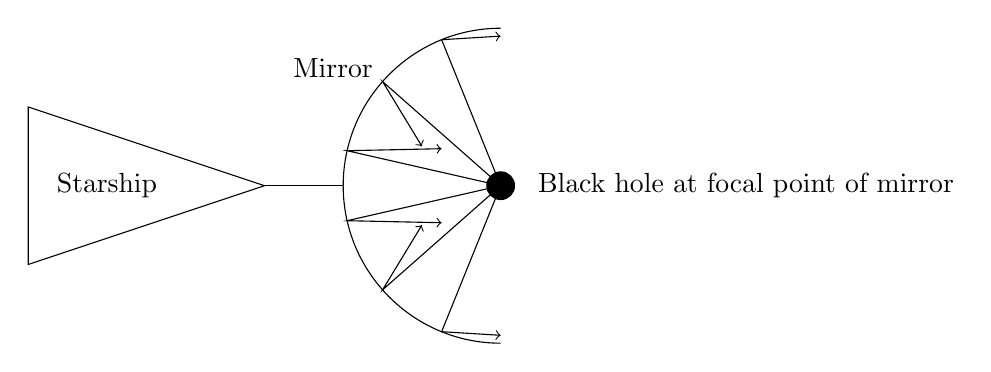
\begin{tikzpicture}
		\coordinate [label=center:Starship] (ShipCentre) at (-2,0);
		\coordinate (ShipTip) at (0,0);
		\coordinate (ShipTopLeft) at (-3,1);
		\coordinate (ShipBottomLeft) at (-3,-1);
		\coordinate [label={[label distance=1em] right:Black hole at focal point of mirror}] (BlackHole) at (3,0);
		\coordinate [label=above left:Mirror] (Mirror) at (1.5,1.25);

		\draw (ShipTopLeft) -- (ShipTip) -- (ShipBottomLeft) -- cycle;

		\draw (3,2) arc (90:270:2);

		\draw (ShipTip) -- (1,0);

		\draw [->] (BlackHole) -- (2.25,1.854049622) -- (3,1.9);
		\draw [->] (BlackHole) -- (2.25,-1.854049622) -- (3,-1.9);

		\draw [->] (BlackHole) -- (1.5,1.322875656) -- (2,0.5);
		\draw [->] (BlackHole) -- (1.5,-1.322875656) -- (2,-0.5);

		\draw [->] (BlackHole) -- (1.05,0.4444097209) -- (2.25,0.47);
		\draw [->] (BlackHole) -- (1.05,-0.4444097209) -- (2.25,-0.47);

		\filldraw[black] (BlackHole) circle (5pt);
	\end{tikzpicture}
\end{figure}
